\begin{document}

\subsection{Lokálne projekty}
\subsubsection{Získavanie dát z rakúskych staníc pomocou Node-Red}
Zo stránky \url{http://sfws.lfrz.at/json.php} je možné získavať dáta dávkového ekvivalentu pod parametrom \say{$v$}. Na stránke je popis ako získavať údaje. Uvádzam príklad výsledného linku ako získať údaje za posledný týždeň: \\
\small{\textit{\url{http://sfws.lfrz.at/json.php?command=getstationdata&stationcode=AT0103&a=7&b=0}}}\\
Dáta sú získané pomocou \textit{GET parametrov}. 


\begin{multicols}{2}
    \begin{description}
        \item[command] - príkaz pre získanie niekoľko druhov údajov
        \item[getstation] - skratka meracej stanice
        \item[a] - počet dní od začiatku merania
        \item[b] - počet dní od konca merania
    \end{description}
\end{multicols}
Vrátené parametre obsahujú pole objektov v JSON formáte. Objekt sa skladá z troch parametrov:
\begin{multicols}{2}
\begin{description}
        \item[d] - časový údaj merania v UNIX TIMESTAMP formáte
        \item[v] - dávkový ekvivalent
        \item[c] - číslo farby pre graf
\end{description}
\end{multicols}
\newpage
Čas UNIX TIMESTAMP sa môže líšiť od lokálneho času pre prípadný prevod som použil uzol s funkciou:
\begin{lstlisting}[style=htmlcssjs]
    msg.payload = JSON.parse(msg.payload)
    msg.payload.v.forEach( (element) => {
      let seventys = new Date(1970,0,1);
        seventys.setSeconds(element.d);
        console.log(seventys);
    element.d2 = new Date(seventys).toLocaleString();
    })
    return msg;
\end{lstlisting}


\begin{figure}[h!]
    \centering
    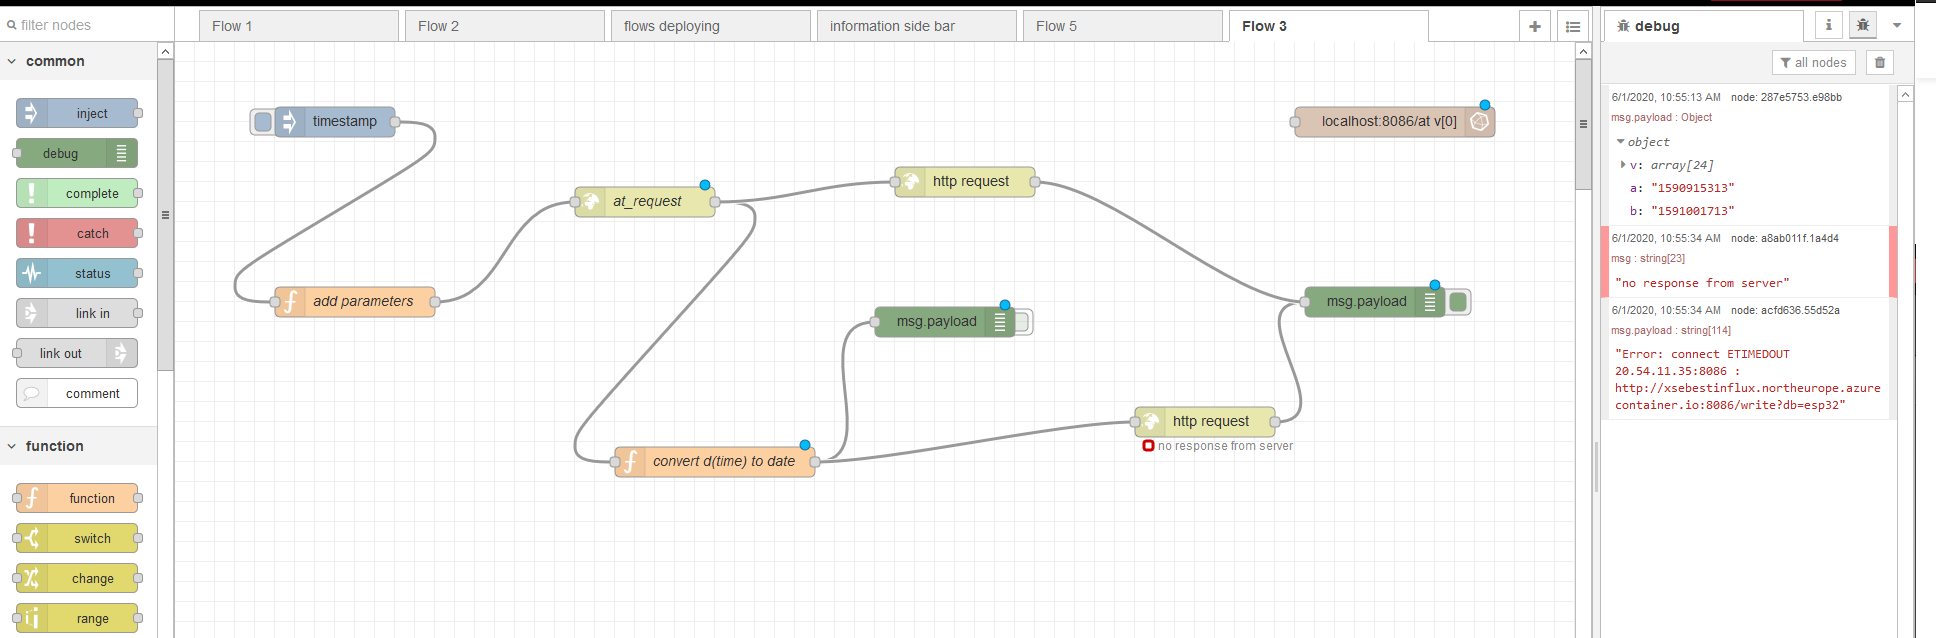
\includegraphics[width=0.8\textwidth]{images/node_red_at.png}
    \caption{Tok tvorený s uzlami pre získavanie dát z AT staníc}
    \label{fig:node_red_at}
\end{figure}

\subsubsection{Inštalácia Docker na lokálnom počítači}
Pre použite kontajnerov som si pripravil prostredie Docker. Snažil som nájsť alebo vytvoriť vhodný Dockefile s prostredím, ktoré sa nachádzalo na QNAPe. Nakoniec som sa uspokojil s image z githubu \url{https://github.com/philhawthorne/docker-influxdb-grafana}, ktorý obsahuje Grafanu, InfluxDB a ešte naviac obsahuje Chronograf, ktorí by mohol byť tiež využitý pre niektoré vizualizácie. Vhodné by bolo aj upraviť aj samotný Dockerfile, a upraviť si ho podľa vlastných potrieb, ale je treba si doštudovať príkazy používané v Dockerfile. Napríklad podľa týchto 2 návodov.
\begin{itemize}
    \item \url{https://docs.docker.com/engine/reference/builder/}
    \item \url{https://rominirani.com/docker-tutorial-series-a7e6ff90a023}
\end{itemize}

\subsubsection{Meranie pomocou teploty a vlhkosti}
Na meranie som využil podobný typ vývojovej dosky, aká sa používala v laboratóriu. Išlo o Heltec LoRaWAN32 s mikrokontrolérom ESP32 a senzorom SHT21 pre meranie vlhkosti a teploty. Podľa návodu \url{https://github.com/espressif/esptool} som nainštaloval MicroPython do vývojovej dosky. Ako vývojove prostredie som používal Visual Studio Code. Bolo nutné doinštalovať Python 3, Pymakr rozšírenie do Visual Studio Code, pomocou ktorého bolo možné zavádzať kód do dosky. Pre vývojový kód som použil približne rovnaký zdrojový kód, aký používali zariadenia v laboratóriu. Bolo treba len nastaviť vývojovej doske pripojenie na sieť, InfluxDB Server a zopár drobností.
Namerané dáta som skúšal posielať do lokálne bežiacich aplikácií (InfluxDB, Grafana, Docker)

\end{document}
